\documentclass[tikz, border=10pt]{standalone}
\usetikzlibrary{automata, positioning, arrows.meta}

\begin{document}
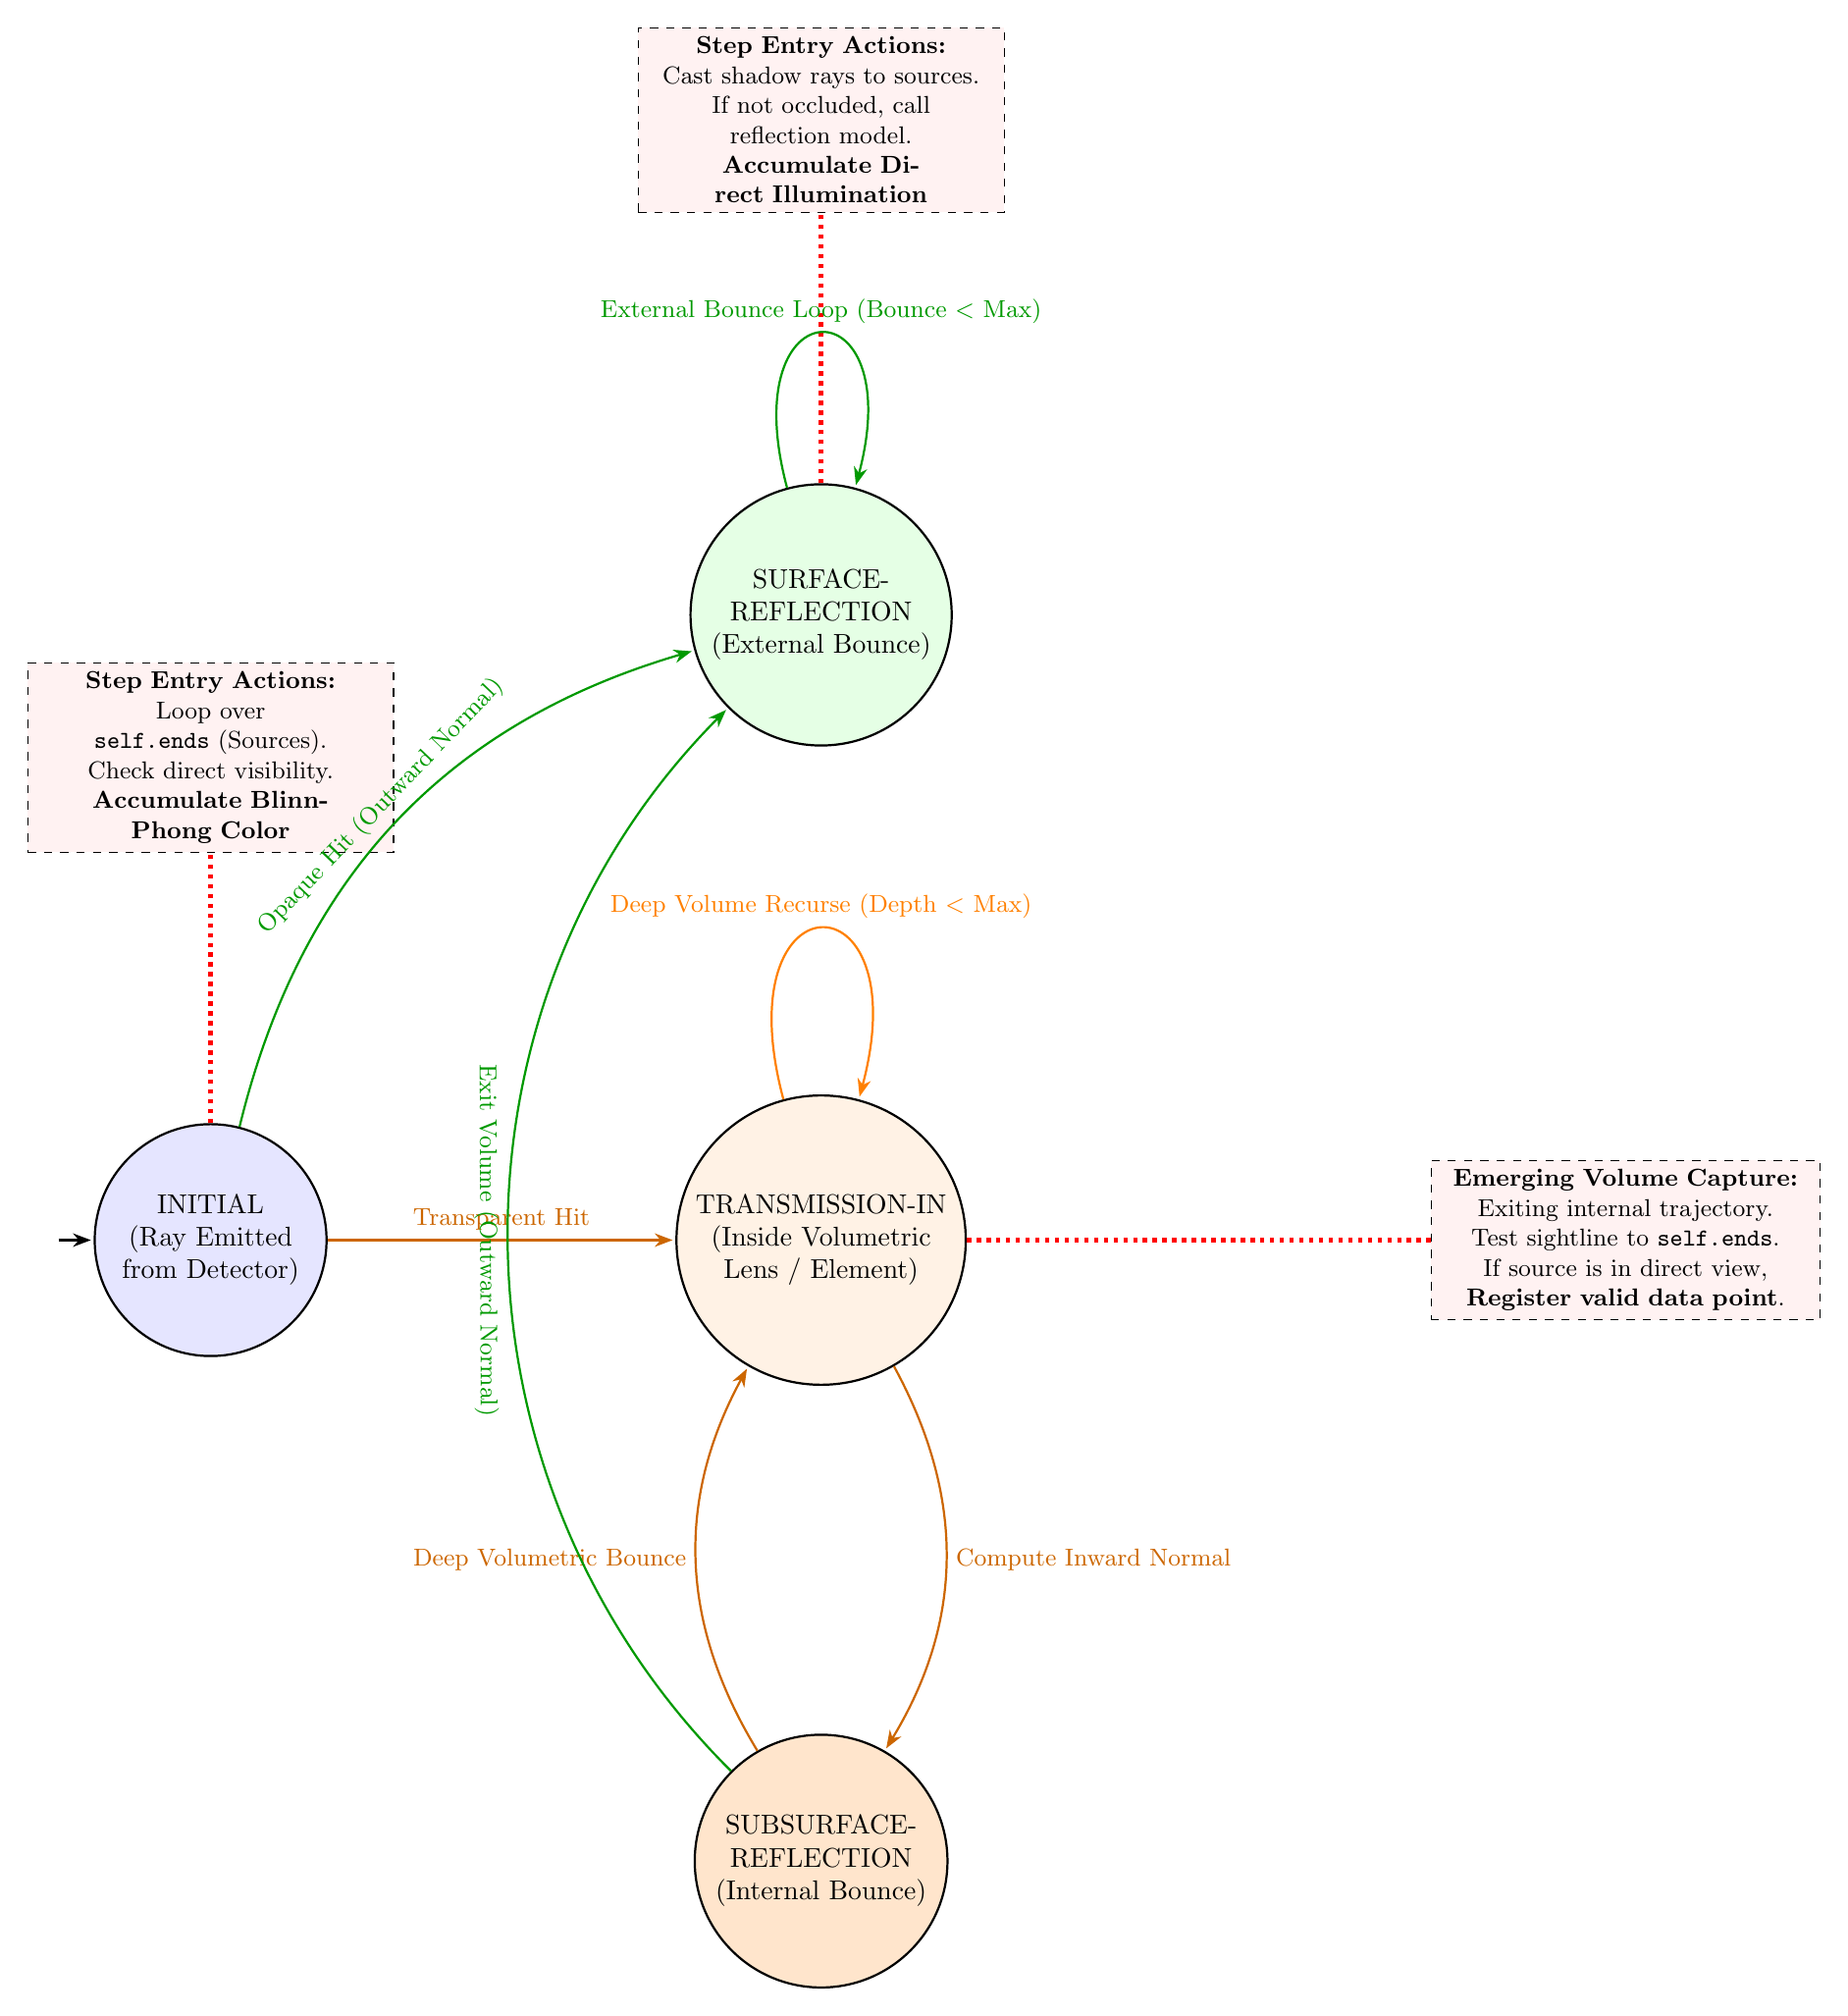
\begin{tikzpicture}[
    >=Stealth,
    node distance=4.5cm,
    every state/.style={thick, fill=blue!10, minimum size=3.0cm, align=center},
    initial text=,
    every edge/.style={draw, ->, thick, shorten >=1pt}
]

    % --- TOPOLOGICAL NODES (Identical Style Grid) ---
    \node[state, initial, initial where=left] (init) {INITIAL\\(Ray Emitted\\from Detector)};
    
    % Volumetric (Transmission) States
    \node[state, right=of init, fill=orange!10] (trans_in) {TRANSMISSION-IN\\(Inside Volumetric\\Lens / Element)};
    \node[state, below=of trans_in, fill=orange!20] (sub_ref) {SUBSURFACE-\\REFLECTION\\(Internal Bounce)};
    
    % Surface (Reflection) States
    \node[state, above=of trans_in, fill=green!10] (surf_ref) {SURFACE-\\REFLECTION\\(External Bounce)};

    % --- REVERSE TRACE EVALUATION OVERLAYS ---
    \node[draw, dashed, fill=red!5, text width=4.5cm, align=center, font=\small, above=of init, yshift=-1cm] (init_eval) 
        {\textbf{Step Entry Actions:}\\Loop over \texttt{self.ends} (Sources).\\Check direct visibility.\\\textbf{Accumulate Blinn-Phong Color}};
        
    \node[draw, dashed, fill=red!5, text width=4.5cm, align=center, font=\small, above=of surf_ref, yshift=-1cm] (surf_eval) 
        {\textbf{Step Entry Actions:}\\Cast shadow rays to sources.\\If not occluded, call reflection model.\\\textbf{Accumulate Direct Illumination}};

    % NEW CORRECTED OVERLAY: Captures data points when rays emerge from internal paths
    \node[draw, dashed, fill=red!5, text width=4.8cm, align=center, font=\small, right=of trans_in, xshift=1.5cm] (emerge_eval)
        {\textbf{Emerging Volume Capture:}\\Exiting internal trajectory.\\Test sightline to \texttt{self.ends}.\\If source is in direct view,\\\textbf{Register valid data point}.};

    % Visual anchor connecting wires
    \draw[dotted, red, ultra thick] (init) -- (init_eval);
    \draw[dotted, red, ultra thick] (surf_ref) -- (surf_eval);
    \draw[dotted, red, ultra thick] (trans_in.east) -- (emerge_eval.west);

    % --- TRANSITIONS & LOGIC FLOW ---
    \path[->] 
        (init) edge[bend left, green!60!black] node[above, sloped, font=\small] {Opaque Hit (Outward Normal)} (surf_ref)
        (init) edge[orange!80!black] node[above, font=\small] {Transparent Hit} (trans_in);

    % Volumetric Loops & Exits
    \path[->]
        (trans_in) edge[loop above, orange] node[above, font=\small] {Deep Volume Recurse (Depth $<$ Max)} (trans_in)
        (trans_in) edge[bend left, orange!80!black] node[right, font=\small] {Compute Inward Normal} (sub_ref)
        (sub_ref) edge[bend left, orange!80!black] node[left, font=\small] {Deep Volumetric Bounce} (trans_in)
        (sub_ref) edge[bend left=45, green!60!black] node[below, sloped, font=\small] {Exit Volume (Outward Normal)} (surf_ref);

    % Surface Loops
    \path[->]
        (surf_ref) edge[loop above, green!60!black] node[above, font=\small] {External Bounce Loop (Bounce $<$ Max)} (surf_ref);

\end{tikzpicture}
\end{document}
